\hypertarget{ux6570ux636eux7c7bux578bux548cux53d8ux91cf}{%
\subsection{数据类型和变量}\label{ux6570ux636eux7c7bux578bux548cux53d8ux91cf}}

\hypertarget{ux6570ux636eux7c7bux578b}{%
\subsubsection{数据类型}\label{ux6570ux636eux7c7bux578b}}

计算机顾名思义就是可以做数学计算的机器,因此,计算机程序理所当然地可以处理各种数值。但是,计算机能处理的远不止数值,还可以处理文本、图形、音频、视频、网页等各种各样的数据,不同的数据,需要定义不同的数据类型。在
Python 中,能够直接处理的数据类型有以下几种:

\hypertarget{ux6574ux6570}{%
\paragraph{整数}\label{ux6574ux6570}}

Python
可以处理任意大小的整数,当然包括负整数,在程序中的表示方法和数学上的写法一模一样,例如:\texttt{1},\texttt{100},\texttt{-8080},\texttt{0},等等。

计算机由于使用二进制,所以,有时候用十六进制表示整数比较方便,十六进制用\texttt{0x}前缀和
0-9,a-f 表示,例如:\texttt{0xff00},\texttt{0xa5b4c3d2},等等。

对于很大的数,例如\texttt{10000000000},很难数清楚 0 的个数。Python
允许在数字中间以\texttt{\_}分隔,因此,写成\texttt{10\_000\_000\_000}和\texttt{10000000000}是完全一样的。十六进制数也可以写成\texttt{0xa1b2\_c3d4}。

\hypertarget{ux6d6eux70b9ux6570}{%
\paragraph{浮点数}\label{ux6d6eux70b9ux6570}}

浮点数也就是小数,之所以称为浮点数,是因为按照科学记数法表示时,一个浮点数的小数点位置是可变的,比如,1.23x109
和 12.3x108
是完全相等的。浮点数可以用数学写法,如\texttt{1.23},\texttt{3.14},\texttt{-9.01},等等。但是对于很大或很小的浮点数,就必须用科学计数法表示,把
10 用 e 替代,1.23x109
就是\texttt{1.23e9},或者\texttt{12.3e8},0.000012
可以写成\texttt{1.2e-5},等等。

整数和浮点数在计算机内部存储的方式是不同的,整数运算永远是精确的(除法难道也是精确的?是的!),而浮点数运算则可能会有四舍五入的误差。

\hypertarget{ux5b57ux7b26ux4e32}{%
\paragraph{字符串}\label{ux5b57ux7b26ux4e32}}

字符串是以单引号\texttt{\textquotesingle{}}或双引号\texttt{"}括起来的任意文本,比如\texttt{\textquotesingle{}abc\textquotesingle{}},\texttt{"xyz"}等等。请注意,\texttt{\textquotesingle{}\textquotesingle{}}或\texttt{""}本身只是一种表示方式,不是字符串的一部分,因此,字符串\texttt{\textquotesingle{}abc\textquotesingle{}}只有\texttt{a},\texttt{b},\texttt{c}这
3
个字符。如果\texttt{\textquotesingle{}}本身也是一个字符,那就可以用\texttt{""}括起来,比如\texttt{"I\textquotesingle{}m\ OK"}包含的字符是\texttt{I},\texttt{\textquotesingle{}},\texttt{m},空格,\texttt{O},\texttt{K}这
6 个字符。

如果字符串内部既包含\texttt{\textquotesingle{}}又包含\texttt{"}怎么办?可以用转义字符\texttt{\textbackslash{}}来标识,比如:

\begin{pythoncode}
'I\'m \"OK\"!'
\end{pythoncode}

表示的字符串内容是:

\begin{pythoncode}
I'm "OK"!
\end{pythoncode}

转义字符 \texttt{\textbackslash{}}
可以转义很多字符,比如\texttt{\textbackslash{}n}表示换行,\texttt{\textbackslash{}t}表示制表符,字符\texttt{\textbackslash{}}本身也要转义,所以\texttt{\textbackslash{}\textbackslash{}}表示的字符就是\texttt{\textbackslash{}},可以在
Python 的交互式命令行用\texttt{print()}打印字符串看看:

\begin{pythoncode}
>>> print('I\'m ok.')
I'm ok.
>>> print('I\'m learning\nPython.')
I'm learning
Python.
>>> print('\\\n\\')
\
\
\end{pythoncode}

如果字符串里面有很多字符都需要转义,就需要加很多\texttt{\textbackslash{}},为了简化,Python
还允许用\texttt{r\textquotesingle{}\textquotesingle{}}表示\texttt{\textquotesingle{}\textquotesingle{}}内部的字符串默认不转义,可以自己试试:

\begin{pythoncode}
>>> print('\\\t\\')
\       \
>>> print(r'\\\t\\')
\\\t\\
\end{pythoncode}

如果字符串内部有很多换行,用\texttt{\textbackslash{}n}写在一行里不好阅读,为了简化,Python
允许用\texttt{\textquotesingle{}\textquotesingle{}\textquotesingle{}...\textquotesingle{}\textquotesingle{}\textquotesingle{}}的格式表示多行内容,可以自己试试:

\begin{pythoncode}
>>> print('''line1
... line2
... line3''')
line1
line2
line3
\end{pythoncode}

上面是在交互式命令行内输入,注意在输入多行内容时,提示符由\texttt{\textgreater{}\textgreater{}\textgreater{}}变为\texttt{...},提示你可以接着上一行输入,注意\texttt{...}是提示符,不是代码的一部分:

\begin{pythoncode}
┌────────────────────────────────────────────────────────┐
│Command Prompt - python                           _ □ x │
├────────────────────────────────────────────────────────┤
│>>> print('''line1                                      │
│... line2                                               │
│... line3''')                                           │
│line1                                                   │
│line2                                                   │
│line3                                                   │
│                                                        │
│>>> _                                                   │
│                                                        │
│                                                        │
│                                                        │
└────────────────────────────────────────────────────────┘
\end{pythoncode}

当输入完结束符\texttt{\textasciigrave{}\textasciigrave{}\textasciigrave{}}和括号\texttt{)}后,执行该语句并打印结果。

如果写成程序并存为\texttt{.py}文件,就是:

\begin{pythoncode}
print('''line1
line2
line3''')
\end{pythoncode}

多行字符串\texttt{\textquotesingle{}\textquotesingle{}\textquotesingle{}...\textquotesingle{}\textquotesingle{}\textquotesingle{}}还可以在前面加上\texttt{r}使用,请自行测试:

\begin{pythoncode}
# -*- coding: utf-8 -*-
\end{pythoncode}

\hypertarget{ux5e03ux5c14ux503c}{%
\paragraph{布尔值}\label{ux5e03ux5c14ux503c}}

布尔值和布尔代数的表示完全一致,一个布尔值只有\texttt{True}、\texttt{False}两种值,要么是\texttt{True},要么是\texttt{False},在
Python
中,可以直接用\texttt{True}、\texttt{False}表示布尔值(请注意大小写),也可以通过布尔运算计算出来:

\begin{pythoncode}
>>> True
True
>>> False
False
>>> 3 > 2
True
>>> 3 > 5
False
\end{pythoncode}

布尔值可以用\texttt{and}、\texttt{or}和\texttt{not}运算。

\texttt{and}运算是与运算,只有所有都为\texttt{True},\texttt{and}运算结果才是\texttt{True}:

\begin{pythoncode}
>>> True and True
True
>>> True and False
False
>>> False and False
False
>>> 5 > 3 and 3 > 1
True
\end{pythoncode}

\texttt{or}运算是或运算,只要其中有一个为\texttt{True},\texttt{or}运算结果就是\texttt{True}:

\begin{pythoncode}
>>> True or True
True
>>> True or False
True
>>> False or False
False
>>> 5 > 3 or 1 > 3
True
\end{pythoncode}

\texttt{not}运算是非运算,它是一个单目运算符,把\texttt{True}变成\texttt{False},\texttt{False}变成\texttt{True}:

\begin{pythoncode}
>>> not True
False
>>> not False
True
>>> not 1 > 2
True
\end{pythoncode}

布尔值经常用在条件判断中,比如:

\begin{pythoncode}
if age >= 18:
    print('adult')
else:
    print('teenager')
\end{pythoncode}

\hypertarget{ux7a7aux503c}{%
\paragraph{空值}\label{ux7a7aux503c}}

空值是 Python
里一个特殊的值,用\texttt{None}表示。\texttt{None}不能理解为\texttt{0},因为\texttt{0}是有意义的,而\texttt{None}是一个特殊的空值。

此外,Python
还提供了列表、字典等多种数据类型,还允许创建自定义数据类型,我们后面会继续讲到。

\hypertarget{ux53d8ux91cf}{%
\subsubsection{变量}\label{ux53d8ux91cf}}

变量的概念基本上和初中代数的方程变量是一致的,只是在计算机程序中,变量不仅可以是数字,还可以是任意数据类型。

变量在程序中就是用一个变量名表示了,变量名必须是大小写英文、数字和
\texttt{\_} 的组合,且不能用数字开头,比如:

\begin{pythoncode}
a = 1
\end{pythoncode}

变量\texttt{a}是一个整数。

\begin{pythoncode}
t_007 = 'T007'
\end{pythoncode}

变量\texttt{t\_007}是一个字符串。

\begin{pythoncode}
Answer = True
\end{pythoncode}

变量\texttt{Answer}是一个布尔值\texttt{True}。

在 Python
中,等号\texttt{=}是赋值语句,可以把任意数据类型赋值给变量,同一个变量可以反复赋值,而且可以是不同类型的变量,例如:

\begin{pythoncode}
# -*- coding: utf-8 -*-
\end{pythoncode}

这种变量本身类型不固定的语言称之为\emph{动态语言},与之对应的是\emph{静态语言}。静态语言在定义变量时必须指定变量类型,如果赋值的时候类型不匹配,就会报错。例如
Java 是静态语言,赋值语句如下(// 表示注释):

\begin{pythoncode}
int a = 123; 
a = "ABC"; 
\end{pythoncode}

和静态语言相比,动态语言更灵活,就是这个原因。

请不要把赋值语句的等号等同于数学的等号。比如下面的代码:

\begin{pythoncode}
x = 10
x = x + 2
\end{pythoncode}

如果从数学上理解\texttt{x\ =\ x\ +\ 2}那无论如何是不成立的,在程序中,赋值语句先计算右侧的表达式\texttt{x\ +\ 2},得到结果\texttt{12},再赋给变量\texttt{x}。由于\texttt{x}之前的值是\texttt{10},重新赋值后,\texttt{x}的值变成\texttt{12}。

最后,理解变量在计算机内存中的表示也非常重要。当我们写:

\begin{pythoncode}
a = 'ABC'
\end{pythoncode}

时,Python 解释器干了两件事情:

\begin{enumerate}
\def\labelenumi{\arabic{enumi}.}
\item
  在内存中创建了一个\texttt{\textquotesingle{}ABC\textquotesingle{}}的字符串;
\item
  在内存中创建了一个名为\texttt{a}的变量,并把它指向\texttt{\textquotesingle{}ABC\textquotesingle{}}。
\end{enumerate}

也可以把一个变量\texttt{a}赋值给另一个变量\texttt{b},这个操作实际上是把变量\texttt{b}指向变量\texttt{a}所指向的数据,例如下面的代码:

\begin{pythoncode}
# -*- coding: utf-8 -*-
\end{pythoncode}

最后一行打印出变量\texttt{b}的内容到底是\texttt{\textquotesingle{}ABC\textquotesingle{}}呢还是\texttt{\textquotesingle{}XYZ\textquotesingle{}}?如果从数学意义上理解,就会错误地得出\texttt{b}和\texttt{a}相同,也应该是\texttt{\textquotesingle{}XYZ\textquotesingle{}},但实际上\texttt{b}的值是\texttt{\textquotesingle{}ABC\textquotesingle{}},让我们一行一行地执行代码,就可以看到到底发生了什么事:

执行\texttt{a\ =\ \textquotesingle{}ABC\textquotesingle{}},解释器创建了字符串\texttt{\textquotesingle{}ABC\textquotesingle{}}和变量\texttt{a},并把\texttt{a}指向\texttt{\textquotesingle{}ABC\textquotesingle{}}:

 
 \begin{figure}[htp]
	\centering
	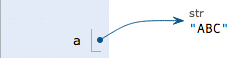
\includegraphics[width=0.6\linewidth]{fig/9237918782554560.png}
\end{figure}


执行\texttt{b\ =\ a},解释器创建了变量\texttt{b},并把\texttt{b}指向\texttt{a}指向的字符串\texttt{\textquotesingle{}ABC\textquotesingle{}}:

 
 \begin{figure}[htp]
	\centering
	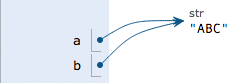
\includegraphics[width=0.6\linewidth]{fig/9237920586134400.png}
\end{figure}


执行\texttt{a\ =\ \textquotesingle{}XYZ\textquotesingle{}},解释器创建了字符串'XYZ',并把\texttt{a}的指向改为\texttt{\textquotesingle{}XYZ\textquotesingle{}},但\texttt{b}并没有更改:

 
 \begin{figure}[htp]
	\centering
	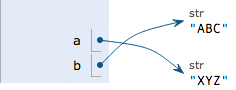
\includegraphics[width=0.6\linewidth]{fig/9237921916377600.png}
\end{figure}


所以,最后打印变量\texttt{b}的结果自然是\texttt{\textquotesingle{}ABC\textquotesingle{}}了。

\hypertarget{ux5e38ux91cf}{%
\subsubsection{常量}\label{ux5e38ux91cf}}

所谓常量就是不能变的变量,比如常用的数学常数π就是一个常量。在 Python
中,通常用全部大写的变量名表示常量:

\begin{pythoncode}
PI = 3.14159265359
\end{pythoncode}

但事实上\texttt{PI}仍然是一个变量,Python
根本没有任何机制保证\texttt{PI}不会被改变,所以,用全部大写的变量名表示常量只是一个习惯上的用法,如果你一定要改变变量\texttt{PI}的值,也没人能拦住你。

最后解释一下整数的除法为什么也是精确的。在 Python
中,有两种除法,一种除法是\texttt{/}:

\begin{pythoncode}
>>> 10 / 3
3.3333333333333335
\end{pythoncode}

\texttt{/}除法计算结果是浮点数,即使是两个整数恰好整除,结果也是浮点数:

\begin{pythoncode}
>>> 9 / 3
3.0
\end{pythoncode}

还有一种除法是\texttt{//},称为地板除,两个整数的除法仍然是整数:

\begin{pythoncode}
>>> 10 
3
\end{pythoncode}

你没有看错,整数的地板除\texttt{//}永远是整数,即使除不尽。要做精确的除法,使用\texttt{/}就可以。

因为\texttt{//}除法只取结果的整数部分,所以 Python
还提供一个余数运算,可以得到两个整数相除的余数:

\begin{pythoncode}
>>> 10 % 3
1
\end{pythoncode}

无论整数做\texttt{//}除法还是取余数,结果永远是整数,所以,整数运算结果永远是精确的。

\hypertarget{ux7ec3ux4e60}{%
\subsubsection{练习}\label{ux7ec3ux4e60}}

请打印出以下变量的值:

\begin{pythoncode}
# -*- coding: utf-8 -*-
n = 123
f = 456.789
s1 = 'Hello, world'
s2 = 'Hello, \'Adam\''
s3 = r'Hello, "Bart"'
s4 = r'''Hello,
Lisa!'''
\end{pythoncode}

\hypertarget{ux5c0fux7ed3}{%
\subsubsection{小结}\label{ux5c0fux7ed3}}

Python 支持多种数据类型,在计算机内部,可以把任何数据都看成一个
``对象'',而变量就是在程序中用来指向这些数据对象的,对变量赋值就是把数据和变量给关联起来。

对变量赋值\texttt{x\ =\ y}是把变量\texttt{x}指向真正的对象,该对象是变量\texttt{y}所指向的。随后对变量\texttt{y}的赋值\emph{不影响}变量\texttt{x}的指向。

注意:Python
的整数没有大小限制,而某些语言的整数根据其存储长度是有大小限制的,例如
Java 对 32 位整数的范围限制在\texttt{-2147483648}-\texttt{2147483647}。

Python
的浮点数也没有大小限制,但是超出一定范围就直接表示为\texttt{inf}(无限大)。

